\documentclass[12pt,a4paper]{article}
\usepackage{amsmath}
\usepackage{amsfonts}
\usepackage{amssymb}
\usepackage{graphicx}
\usepackage{secdot}
\usepackage[left=2cm,right=2cm,top=2cm,bottom=2cm]{geometry}

\author{Shibayan Biswas, AE21B109,\\ Department of Aerospace Engineering,\\ IIT Madras}

\title{Case Study (Part - II)}

\begin{document}

\maketitle

\hline

\section{Problem I:}
This is the first problem for our project. Given below is the statement and explanation for the given problem:
\subsection{Statement:}
Your Friend has developed the Product and he wants to establish the product startup and he is searching for a perfect location where getting the investment has a high chance. But due to its financial restriction, he can choose only between three locations - Bangalore, Mumbai, and NCR. As a friend, you want to help your friend deciding the location. NCR include Gurgaon, Noida and New Delhi. Find the location where the most number of funding is done. That means, find the location where startups has received funding maximum number of
times. Plot the bar graph between location and number of funding. Take city name "Delhi" as "New Delhi". Check the case-sensitiveness of cities also. That means, at some place instead of "Bangalore", "bangalore" is given. Take city name as "Bangalore". For few startups multiple locations are given, one Indian and one Foreign. Consider the startup if any one of the cities lies in given locations.
\begin{figure}[!ht]
	\begin{center}
			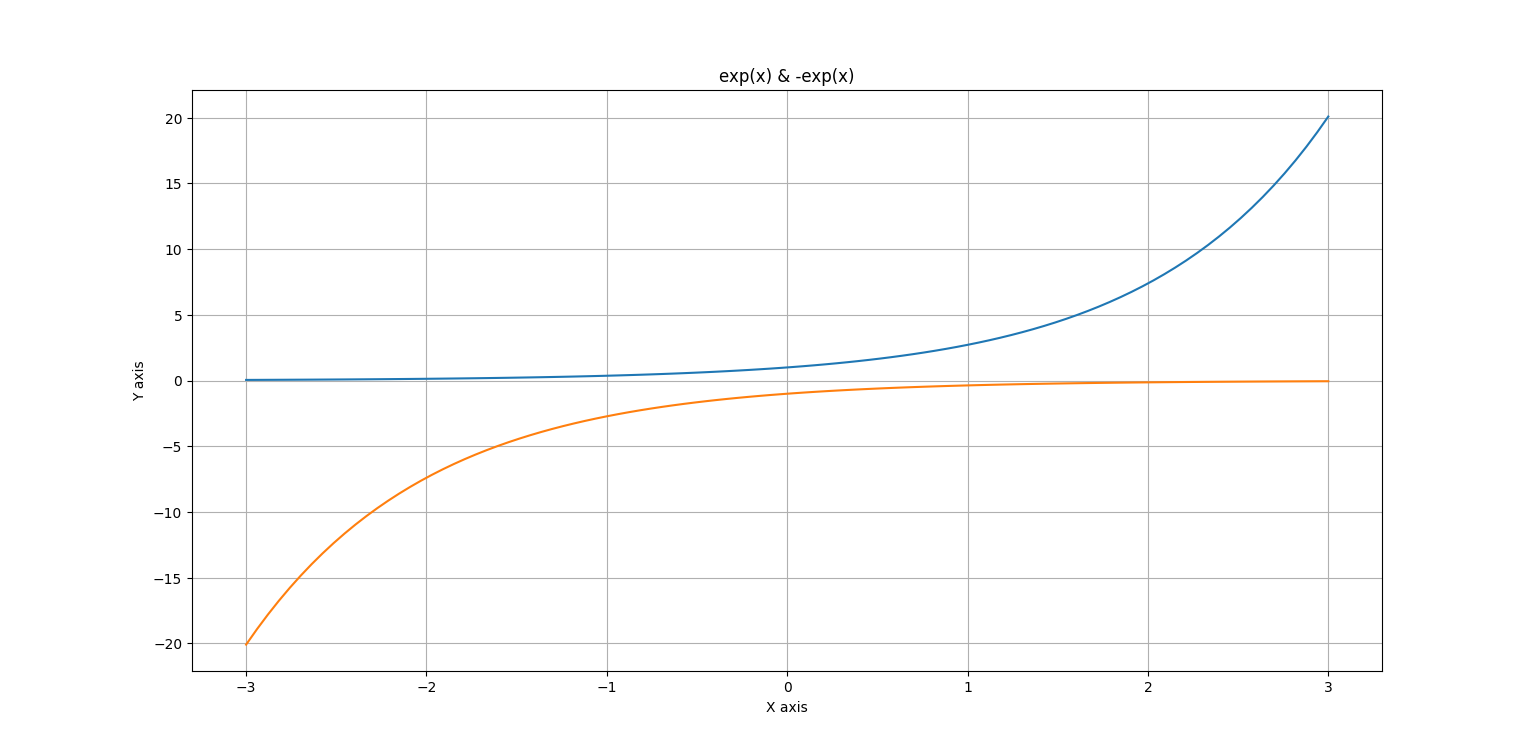
\includegraphics[scale=0.8]{Figure_1.png}
	\end{center}
\end{figure}
\clearpage
\subsection{Explanation:}
Firstly, I Drop rows having NaN value in "CityLocation" and "AmountInUSD" column in dataset, Separate the Investors who have invested in same startup. then correct spelling mistake in City name after this I select Bangalore, Mumbai and NCR cities. I Find location where the most number of funding is done. I plot bar graph between city and No. of fundings.\\
\\As we see that Bangalore is a city which received maximum number of fundings. So, if anyone wants to open a startup; Bangalore would be the best city to consider. In this case due to financial restriction my friend can only
choose between Bangalore, Mumbai and NCR which includes New Delhi, Gurgaon and Noida. I find the number of funding in each of these cities and draw a Bar Graph between cities and number of fundings. From the above graph I conclude that if he opens his startup in Bangalore then he has a high chance to get the funding maximum
number of times.
\section{Problem II:}
This is the second problem for our project. Given below is the statement and explanation for the given problem:
\subsection{Statement:}
Even after trying for so many times, your friend’s startup could not find the investment. So you decided to take this matter in your hand and try to find the list of investors who probably can invest in your friend’s startup. Your list will increase the chance of your friend startup getting some initial investment by contacting these investors. Find the top 5 investors who have invested maximum number of times (consider repeat investments in one company also). In a startup, multiple investors might have invested. So consider each investor for that startup. Ignore undisclosed investors.
\begin{figure}[!ht]
	\begin{center}
			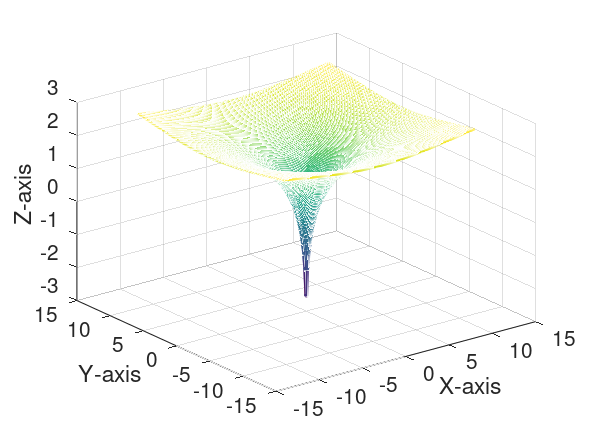
\includegraphics[scale=1.0]{Figure_2.png}
	\end{center}
\end{figure}
\clearpage
\subsection{Explanation:}
In This problem firstly I eliminate rows having NaN values in "InvestorName" column in dataset. Here I have ignored undisclosed Investors from the given dataset. Separate the Investors who have invested in same startup. I plot
Pie graph to show the percentage of investing according to investors.\\
\\So, the solution come out with top 5 investors who have invested maximum number of times. In above pie graph we can see that Sequoia Capital is the Top investor having maximum percentage in investing. So, my friend can contact with these investors.
\section{Problem III:}
This is the third problem for our project. Given below is the statement and explanation for the given problem:
\subsection{Statement:}
After re-analysing the dataset you found out that some investors have invested in the same startup at different number of funding rounds. So before finalising the previous list, you want to improvise it by finding the top 5 investors who have invested in different number of startups. This list will be more helpful than your previous list in finding the investment for your friend startup. Find the top 5 investors who have invested maximum number of times in different companies. That means, if one investor has invested multiple times in one startup, count one for that company. There are many errors in startup names. Ignore correcting all, just handle the important ones - Ola, Flipkart, Oyo and Paytm.
\begin{figure}[!ht]
	\begin{center}
			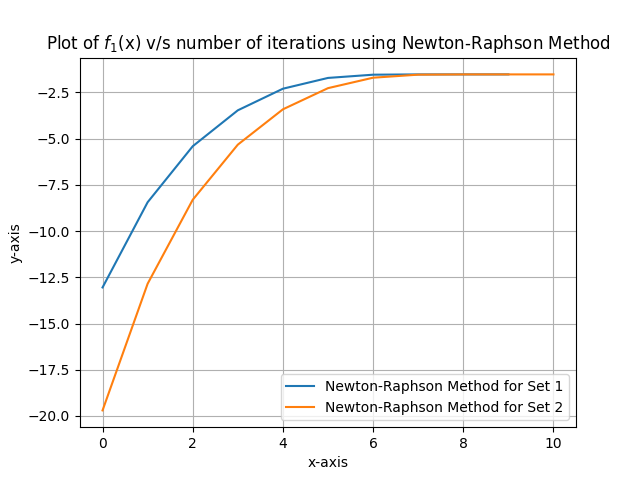
\includegraphics[scale=0.9]{Figure_3.png}
	\end{center}
\end{figure}
\subsection{Explanation:}
Here I eliminate rows having NaN value in "StartupName" and "InvestorsName" column in dataset then correct spelling mistake in startup name and ignore Undisclosed Investors. Separate the multi-investors from same cell in
dataset. Create new dataset having only InvestorsName and StartupName. I find the top 5 investors who have invested maximum number of times in different companies. Plot Bar graph between Top 5 investor and number of investing.\\
\\This is a Bar Graph between Top 5 investors and the number of Investments they did. These top investors information is more helpful than previous problem because in this case we get top investors who are investing more in different startups rather than in a same startup. The Probability of getting the investment from These investors are high because they are investing more in different startups.
\section{Problem IV:}
This is the fourth problem for our project. Given below is the statement and explanation for the given problem:
\subsection{Statement:}
Even after putting so much effort in finding the probable investors, it didn't turn out to be helpful for your friend. So you went to your investor friend to understand the situation better and your investor friend explained to you about the different Investment Types and their features. This new information will be helpful in finding the right investor. Since your friend startup is at an early stage startup, the best-suited investment type would be - Seed Funding and Crowdfunding. Find the top 5 investors who have invested in a different number
of startups and their investment type is Crowdfunding or Seed Funding. Correct spelling of investment types are - "Private Equity", "Seed Funding", "Debt Funding", and "Crowd Funding". Keep an eye for any spelling mi
stake. You can find this by printing unique values from this column. There are many errors in startup names. Ignore correcting all, just handle the important ones - Ola, Flipkart, Oyo and Paytm.
\begin{figure}[!ht]
	\begin{center}
			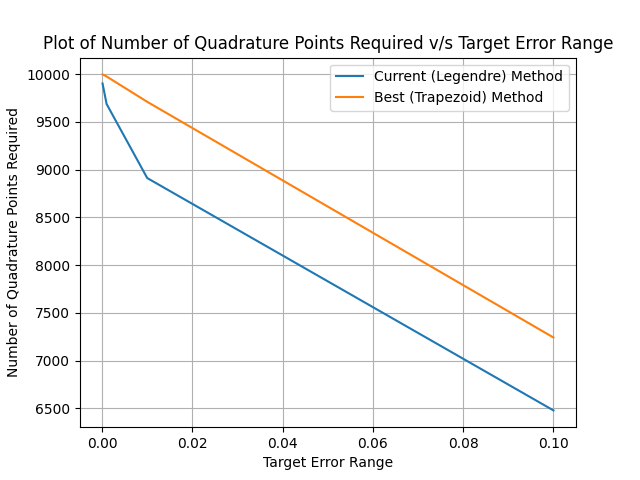
\includegraphics[scale=0.6]{Figure_4.png}
	\end{center}
\end{figure}
\clearpage
\subsection{Explanation:}
Here I eliminate rows having NaN value in "InvestorsName" and "StartupName" column in dataset. Correct spelling mistakes in startup name. Ignored Undisclosed Investors from dataset and Correct spelling mistakes in Investment Type. Select Crowd Funding or Seed Funding from "InvestmentType" and separate investors from a single cell in dataset. Create new dataset having only InvestorsName and StartupName then I find the top 5 investors who have invested in different number of startups. I plot Bar graph between Top investors and their investments.\\
\\According to the graph, These are top investors who invested in startups where investment type is either Crowd Funding or Seed Funding. And also, this is the list of top investors who are interested in the early stage of startups
or newly startups. So, if anyone wants to establish a new startup, then for investment purpose he should consider these top investors.
\section{Problem V:}
This is the fifth problem for our project. Given below is the statement and explanation for the given problem:
\subsection{Statement:}
Due to your immense help, your friend startup successfully got seed funding and it is on the operational mode. Now your friend wants to expand his startup and he is looking for new investors for his startup. Now you again come as a saviour to help your friend and want to create a list of probable new new investors. Before moving forward you remember your investor friend advice that finding the investors by analysing the investment type. Since your friend startup is not in early phase it is in growth stage so the best-suited investment type is Private Equity. Find the top 5 investors who have invested in a different number of startups and their investment type is Private Equity. Correct spelling of investment types are - "Private Equity", "Seed Funding", "Debt Funding", and "Crowd Funding". Keep an eye for any spelling mistake. You can find this by printing unique values from this column. There are many errors in startup names. Ignore correcting all, just handle the important ones - Ola, Flipkart, Oyo and Paytm.
\begin{figure}[!ht]
	\begin{center}
			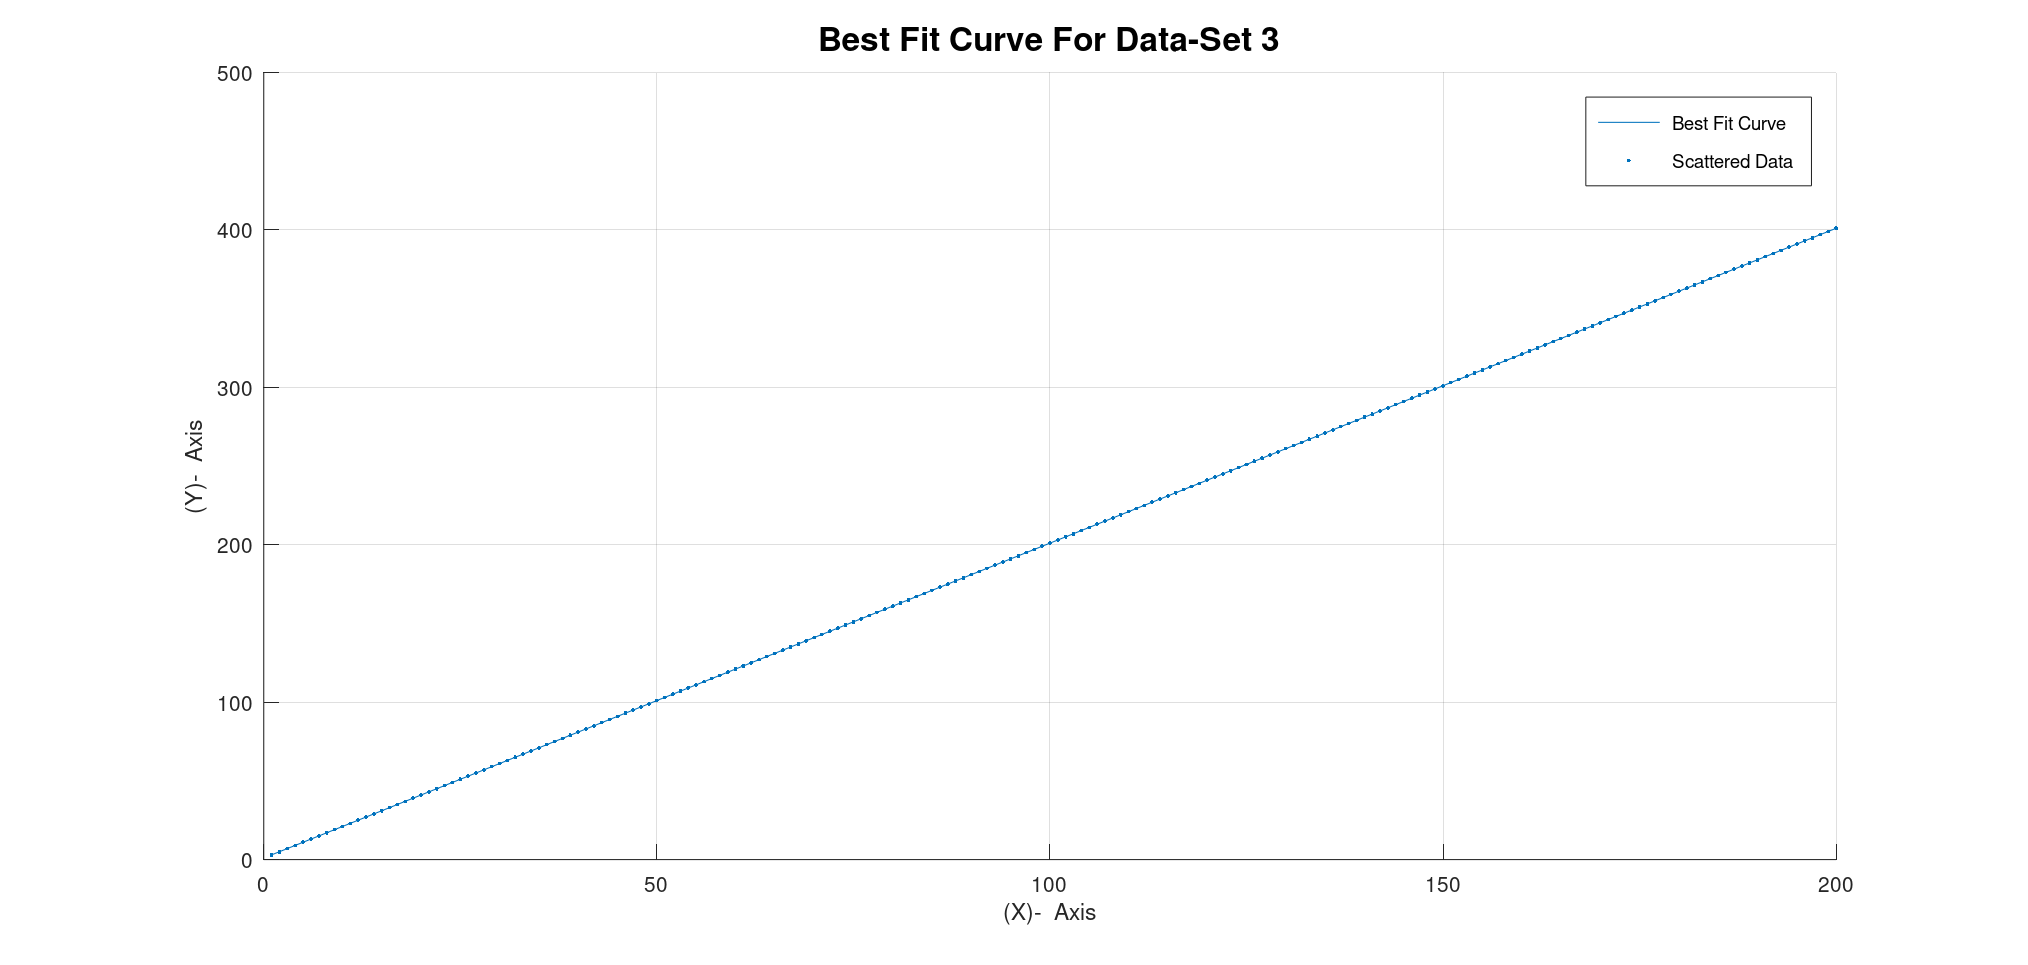
\includegraphics[scale=0.65]{Figure_5.png}
	\end{center}
\end{figure}
\clearpage
\subsection{Explanation:}
Here I eliminate rows having NaN values in "InvestorsName" and "StartupName" column in dataset. I correct Startup Name spelling and ignore undisclosed Investors and correct spelling mistakes in Investment Type. I select only Private Equity as Investment Type. I separate the Investors Name from same cell in dataset. I Create new dataset having only two columns named InvestorsName and StartupName then I find the top 5 investors who
have invested in a different number of startups.I plot bar graph between Top investors and their investment.\\
\\According to the graph, these are the top investors who invested in startups where investment type is Private Equity. And also, this is the list of top investors who are looking to invest in the growth stage of any startup or
established startups. So, if anyone wants new investors for the established startup then he should consider these top investors.
\end{document}
